%% content.tex
%%

%% ==============
\chapter{Algorithm}
\label{ch:Algorithm}
%% ==============

The content chapters of your thesis should of course be renamed. How many chapters you need to write depends on your thesis and cannot be said in general.


\section{Problem Description}
The shortest path problem with driving time constraints consists of a Graph $G=(V,E)$, a set $P \subseteq V$ of parking nodes, a set $R$ of driving time constraints $r_i$ and start and target nodes $s$ and $t$. Each driving time constraint  is defined by a maximum allowed driving time $r_{i,d}$ and a pause time $r_{i,p}$. Thereby, the driving time constraints define a relation $r_i \le r_{i+1}$ with $r_i \le r_j \implies r_{i,d} \le r_{j,d} \land  r_{i,p} \le r_{j,p} \forall i,j$.

Before exceeding a driving time of $r_{i,d}$, the driver must stop and pause for a time of at least $r_{i,p}$. Afterwards, the driver is allowed to drive for a maximum time of $r_{i,d}$ again without stopping. Stops can only take place at nodes $v \in P$.

In many practical applications, the number of different driving time constraints is limited to only one or two constraints, i.e. $|R| = 1$ or  $|R| = 2$. Therefore, we will often only consider one of these special cases.

\subsection{General Approach}
We introduce a labeling algorithm which solves the shortest path problem with driving time constraints. todo

\paragraph{Complexity}
d


\section{A* Variant}
\subsection{Dijkstra's Algorithm with One Driving Time Constraint}
A driving time constraint is a rule which defines a maximum allowed  non-stop driving time $t_d$ and a pause time $t_p$. Before the driving time limit $t_d$ is exceeded, the driver must park at designated parking for a minimum time period of $t_p$ before continuing.

The base algorithm with one driving time constraint extends a Dijkstra search with pruning rules to comply with the constraint. It uses distance labels which it propagates between the nodes. The search operates on a graph $G = (V,E,\omega)$ with the available parking nodes defined as a subset $P \subseteq V$. The search can decide to \emph{park} at a node $v$ if $v \in P$.

Each node $v$ holds a set $L(v)$ of \emph{labels}. Each label at a node $v$ holds two distances $d_0$ and $d_1$ and a link to the previous label. The chain of linked labels represents a unique \emph{path} from $s$ to $v$. A path is characterized by the sequence of visited nodes $v_i$ and a subset of all $v_i \in P$ to describe the parking nodes on the path which were used for parking. The distance $d_0$ describes the distance on the path from the start node $s$ and $d_1$ since the last pause, i.e., the distance from the last node $v_i \in P$ which was used for parking.


\begin{algorithm}[bt]
	\caption{\textsc{CSP}}\label{alg:CSP}

	% Some settings
	\DontPrintSemicolon %dontprintsemicolon
	\SetFuncSty{textsc}
	\SetKwFor{ForAll}{forall}{do}

	% Declaration of data containers and functions
	\SetKwData{Q}{Q}
	\SetKwData{dist}{d}
	\SetKwData{L}{L}
	\SetKwData{pred}{pred}
	\SetKwArray{ds}{ds}
	\SetKwFunction{queueDeleteMin}{deleteMin}
	\SetKwFunction{queueInsert}{insert}
	\SetKwFunction{queueMin}{min}
	\SetKwFunction{queueMinKey}{minKey}
	\SetKwFunction{queueDecreaseKey}{decreaseKey}
	\SetKwFunction{queueContains}{contains}
	\SetKwFunction{listInsert}{insert}
	\SetKwFunction{removeDom}{removeDominated}

	% Algorithm interface
	\KwIn{Graph $G = (V,E,\omega)$, parking nodes $P \subseteq V$, driving time restriction $r$, source node $s \in V$}
	\KwData{Priority queue \Q, per node priority queue \L{$v$} of labels for all $v \in V$}
	\KwOut{Distances \dist{$v$} for all $v \in V$, shortest-path tree of $s$ given by \pred{$\cdot$}}

	% The algorithm
	\BlankLine
	\tcp{Initialization}
	\Q.\queueInsert{$s,(0,0)$}\;
	\L{$s$}.\queueInsert{$(\bot,\bot),(0,0)$}\;
	\BlankLine
	\tcp{Main loop}
	\While{\Q is not empty}
	{
		$u \leftarrow$ \Q.\queueDeleteMin{} \;
		$(d_0, d_1) \leftarrow$ \L{$u$}.\queueMinKey{} \;
		$l \leftarrow$ \L{$u$}.\queueDeleteMin{} \;
		\BlankLine
		\If{\L{$u$} is not empty}
		{
			$k_{dist} \leftarrow$ \L{$u$}.\queueMinKey{} \;
			\Q.\queueInsert{$u$, $k_{dist}$} \;
		}

		\ForAll{ $(u,v) \in E$ }
		{
			\If{$d_0 + \omega(u,v) < r_d$}
			{
				$D \leftarrow \{(d_0 + \omega(u,v), d_1 + \omega(u,v))\}$

				\If{$v \in P$}
				{
					$D$.\listInsert{$(d_0 + \omega(u,v) + r_p, 0)$}
				}

				\ForAll{ $x \in D$ }
				{
					\If{$x$ is not dominated by any label in \L{$v$}}
					{
						\L{$v$}.\removeDom{$x$} \;
						\L{$v$}.\queueInsert{$(l,(u,v)), x$} \;
						\uIf{\Q.\queueContains{v}}
						{
							\Q.\queueDecreaseKey{$v, x$}
						}
						\Else
						{
							\Q.\queueInsert{$v, x$}
						}
					}
				}
			}
		}
	}
\end{algorithm}

\subsection{Potential for Driving Time Constraints}
Given a target node $t$, the CH potential $\pi_{t,ch}$ yields a perfect estimate for the distance $d_{direct}(v,t)$ from $v$ to $t$ without regard for driving time restrictions and pauses. A lower bound for the time $d(v,t)$ from $v$ to $t$ with breaks due to the driving time limit can be calculated by taking the minimum necessary amount of breaks on the shortest path into account:

\[\pi{'}_t(v) = \floor*{ \frac{d_{direct}(v,t)}{t_d} } * t_p + d_{direct}(v,t)\]

A node potential is called \emph{feasible} if it does not overestimate the distance of any edge in the graph, i.e.
\begin{align}
	\label{eq:node_potential_feasibility}
	len(u,v) - pot(u) + pot(v) \ge 0 \quad \forall (u,v) \in E
\end{align}
Following example of a query using the graph in Fig. \ref{fig:graph_infeasible_potential} shows that $\pi{'}_t$ is not feasible. With a driving time limit of 6 and a pause time of 1, the potential here will yield a value $\pi_t(s) = 8$ since the potential includes the minimum required pause time for a path from s to t. Consequently, with $\pi_t(v) = 5$ and $len(s,v) = 2$, $len(s,v) - \pi_t(s) + \pi_t(v) = -1$.

\begin{figure}[hbtp]
	\centering
	\tikzstyle{node}=[circle,inner sep=0.5mm,minimum size=5.25mm,draw = black]
\tikzstyle{bright}=[fill=black!14]
\tikzstyle{dark}=[fill=black!28]
\tikzstyle{lightEdgeStyle}=[black!20]

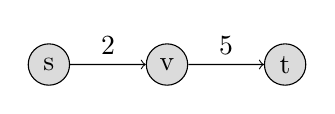
\begin{tikzpicture}[scale=1.5, bend angle = 20]

	% Obere Reihe
	\node(s) at (1,1) [node, bright] {s};
	\node(v) at (2,1) [node, bright] {v};
	\node(t) at (3,1) [node, bright] {t};

	\draw[->] (s) -> node[midway, above]{2} (v);
	\draw[->] (v) -> node[midway, above]{5} (t);
	% \foreach \i [evaluate = \i as \lastNode using \i-1] in {2,3,...,\numberOfNodes}
	% 	{
	% 		\node (Top\i) at (\i,1) [node, bright] {\i}
	% 		edge[<-] (Top\lastNode);
	% 	}


	% % Pfeile nach rechts
	% \pgfmathparse{\numberOfNodes - 2}
	% \foreach \i [evaluate = \i as \nextNode using \i+2] in {1,2,...,\pgfmathresult}
	% 	{
	% 		\foreach \j [count=\nodeIndex from \nextNode] in {\nextNode,...,\numberOfNodes}
	% 			{
	% 				\draw[->, lightEdgeStyle] (Bot\i) to [bend right] (Bot\nodeIndex);
	% 			}
	% 	}

\end{tikzpicture}

	\caption{A graph with the potential to break the potential.}
	\label{fig:graph_infeasible_potential}
\end{figure}

A variant of the potential accounts for the distance $d(p,v)$ with $p$ being the last parking node that was used for a pause to calculate the minimum required pause time on the $v$-$t path$. Since the potential now uses information from a label $l$ with $l \in L(v)$, it no longer is a node potential but also depends on the chosen label at $v$.

\begin{align*}
	\pi_t(l,v) & = \floor*{ \frac{d_{direct}(p,v) + d_{direct}(v,t)}{t_d} } * t_p + d_{direct}(v,t) \\
	           & = \floor*{ \frac{d_1(l) + d_{direct}(v,t)}{t_d} } * t_p + d_{direct}(v,t)
\end{align*}

\begin{definition}
	\label{def:label_potential_feasibility}
	A label potential $pot(l,v)$ with $l \in L(v)$ is feasible if for all $(u,v) \in E$, $l \in L(u)$, and $m \in L(v)$ where $l$ is a direct predecessor of $m$:

	\begin{align}
		len(u,v) - \pi_t(l,u) + \pi_t(m,v) \ge 0
	\end{align}
\end{definition}

\begin{theorem}
	The potential $\pi_t$ is a feasible label potential.
\end{theorem}

\begin{proof}
	Given a Graph $G=(V,E)$ with a set of parking nodes $P \subseteq V$, any edge $(u,v) \in E$, label $l \in L(u)$, $m \in L(v)$ with $l$ is a direct predecessor of m. Let $s,t \in V$ be starting node and target node of a query in G and $p,q \in P \cup \{s\}$.

	\begin{align}
		\begin{split}\label{eq:label_feasibility_proof_1}
			len(u,v) - \pi_t(l,u) + \pi_t  (m,v)                                                                                                                                                                                                       \\
			& =  len(u,v) - \left(\floor*{ \frac{d_1(l) + d_{direct}(u,t)}{t_d} } * t_p + d_{direct}(u,t)\right)                                                                                                                                      \\
			& \phantom{{}=1} +  \floor*{ \frac{d_1(m) + d_{direct}(v,t)}{t_d} } * t_p + d_{direct}(v,t)                                                                                                                                               \\
			& =  \floor*{ \frac{d_1(m) + d_{direct}(v,t)}{t_d} } * t_p - \floor*{ \frac{d_1(l) + d_{direct}(u,t)}{t_d} } * t_p                                                                                                                        \\
			& \phantom{{}=1} + len(u,v) + d_{direct}(v,t) - d_{direct}(u,t)                                                                                                                                                                           \\
			& \ge   \floor*{ \frac{d_1(m) + d_{direct}(v,t)}{t_d} } * t_p - \floor*{ \frac{d_1(l) + d_{direct}(u,t)}{t_d} } * t_p                                                                                                                       \\
			& =  \underbrace{ \floor*{ \frac{d_{direct}(q,v) + d_{direct}(v,t)}{t_d} } * t_p}_\text{min. pause time on q-v-t path}\\
			& \phantom{{}=1} - \underbrace{\floor*{ \frac{d_{direct}(p,u) + d_{direct}(u,t)}{t_d} } * t_p}_\text{min. pause time on p-u-t path}
		\end{split}
	\end{align}

	The nodes $p,q$ represent the last used parking node of the labels $l,m$ or the starting node if no parking node was used. The condition for feasibility of a label potential as in \ref{def:label_potential_feasibility} simplifies to

	\begin{align*}
		\textit{number of breaks on q-v-t path} - \textit{number of breaks on p-u-t path} \ge 0
	\end{align*}

	\emph{Case 1: $u \notin P \land v \notin P$}. Since both $u$ and $v$ are no parking nodes and $l$ is a direct predecessor of $m$, both label used the same parking node for their last pause or did not pause, therefore $q=p$ and

	\begin{align}
		\begin{split}\label{eq:label_feasibility_proof_2}
			d_{direct}(p,u) + d_{direct}(u,t) & = d_{direct}(p,u) + len(u,v) + d_{direct}(v,t) \\
			& = d_{direct}(q,u) + len(u,v) + d_{direct}(v,t) \\
			& = d_{direct}(q,v) + d_{direct}(v,t)
		\end{split}
	\end{align}

	With equations \ref{eq:label_feasibility_proof_1} and \ref{eq:label_feasibility_proof_2} follows $len(u,v) - \pi_t(l,u) + \pi_t(m,v) = 0$ and $\pi_t$ is a feasible label potential.

	\emph{Case 2: $u \in P \land v \notin P$}. In this case, $u = q = p$ and $\pi_t$ is a feasible label potential as shown in case 1.

	\emph{Case 3: $u \notin P \land v \in P$}. In this case, $q \neq p$ and $d_{direct}(q,v) = 0$.

	\begin{align}
		\begin{split}
			\floor*{ \frac{d_{direct}(q,v) + d_{direct}(v,t)}{t_d} } * t_p - \floor*{ \frac{d_{direct}(p,u) + d_{direct}(u,t)}{t_d} } * t_p \\
			= \floor*{ \frac{d_{direct}(v,t)}{t_d} } * t_p - \floor*{ \frac{d_{direct}(p,u) + d_{direct}(u,t)}{t_d} } * t_p
		\end{split}
	\end{align}
\end{proof}
TODO this doesn't add up completly

\begin{lemma}
	The label potential of a label $l$ at a node $v$ is a lower bound for the distance including pauses from $v$ to $t$.
\end{lemma}

\begin{proof}
	Let $p = \langle s=v_0,v_1,...,t=v_k, \rangle$ be a path. With $\pi_t(l_{i-1},v_{i-1}) \ge \pi_t(l_i,v_i) + l(v_{i-1},v_i)$ for all edges on $p$, the total length $l(p)$ of the path must follow $\pi_t(l_k,t) + l(p) \ge \pi_t(l_0,s) \Leftrightarrow l(p) \ge \pi_t(l_0,s) - \pi_t(l_k,t)$. Since $\pi_t(l_k,t) = 0$, $l(p) \ge \pi_t(l_0,s)$ holds.
\end{proof}

\begin{theorem}
	The search can be stopped when the first label at $t$ is removed from the queue.
\end{theorem}

\begin{proof}
	When a label $l$ at $t$ is removed from the queue during a $s$-$t$ query, all remaining label $m$ of a node $v$ in the queue fulfill $d_0(t) + \pi_t(l,t) \le d_0(v) + \pi_t(m,v)$. Assume that $d_0(t)$ is not the shortest distance. Then, an $s$-$t$ path $p = \langle s=v_0,v_1,...,t=v_k, \rangle$ exists which uses at least one unsettled label $m \in L(v_i)$. Since $l$ was already removed from the queue, $d_0(t) = d_0(t) + \pi_t(l,t) \le  d_0(v) + \pi_t(m,v) \le l(p)$.
\end{proof}

% \begin{proof}
% 	Given a Graph $G=(V,E)$ and any path $p = \langle v_0,v_1,...,v_k, \rangle$.
% \end{proof}
% The conditions in which $\pi_t(v)$ is feasible can be derived directly from the requirement for a feasible potential, i.e. $len(u,v) - pot(u) + pot(v) \ge 0$:

% \begin{align*}
% 	len(u,v) - \pi_t(u) + \pi_t  (v)                                                                                                                                                                                         \\
% 	 & =  len(u,v) - \left(\floor*{ \frac{d(p,u) + d_{direct}(u,t)}{t_d} } * t_p + d_{direct}(u,t)\right)                                                                                                                    \\
% 	 & \phantom{{}=1} +  \floor*{ \frac{d(p,v) + d_{direct}(v,t)}{t_d} } * t_p + d_{direct}(v,t)                                                                                                                             \\
% 	 & =  \floor*{ \frac{d(p,v) + d_{direct}(v,t)}{t_d} } * t_p - \floor*{ \frac{d(p,u) + d_{direct}(u,t)}{t_d} } * t_p                                                                                                      \\
% 	 & \phantom{{}=1} + len(u,v) + d_{direct}(v,t) - d_{direct}(u,t)                                                                                                                                                         \\
% 	 & =  \underbrace{ \floor*{ \frac{d(p,v) + d_{direct}(v,t)}{t_d} } * t_p}_\text{min. pause time on s-v-t path} - \underbrace{\floor*{ \frac{d(p,u) + d_{direct}(u,t)}{t_d} } * t_p}_\text{min. pause time on s-u-t path}
% \end{align*}

% The potential therefore is infeasible if the minimum required pause time on an $s$-$t$ path via $u$ is greater than the minimum required pause time on an $s$-$t$ path via $v$. An example graph where this case occurs is given in Fig. \ref{fig:graph_infeasible_potential_2}.
% \begin{figure}[hbtp]
% 	\centering
% 	\tikzstyle{node}=[circle,inner sep=0.5mm,minimum size=5.25mm,draw = black]
\tikzstyle{bright}=[fill=black!14]
\tikzstyle{dark}=[fill=black!28]
\tikzstyle{lightEdgeStyle}=[black!20]

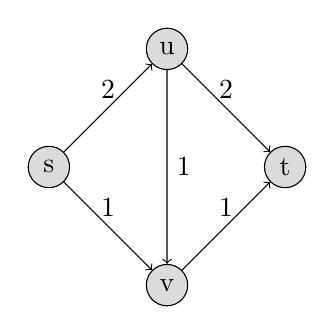
\begin{tikzpicture}[scale=1.5, bend angle = 20]

	% Obere Reihe
	\node(u) at (2,3) [node, bright] {u};
	\node(s) at (1,2) [node, bright] {s};
	\node(t) at (3,2) [node, bright] {t};
	\node(v) at (2,1) [node, bright] {v};

	\draw[->] (s) -> node[midway, above]{2} (u);
	\draw[->] (u) -> node[midway, above]{2} (t);
	\draw[->] (s) -> node[midway, above]{1} (v);
	\draw[->] (v) -> node[midway, above]{1} (t);
	\draw[->] (u) -> node[midway, right]{1} (v);
	% \foreach \i [evaluate = \i as \lastNode using \i-1] in {2,3,...,\numberOfNodes}
	% 	{
	% 		\node (Top\i) at (\i,1) [node, bright] {\i}
	% 		edge[<-] (Top\lastNode);
	% 	}


	% % Pfeile nach rechts
	% \pgfmathparse{\numberOfNodes - 2}
	% \foreach \i [evaluate = \i as \nextNode using \i+2] in {1,2,...,\pgfmathresult}
	% 	{
	% 		\foreach \j [count=\nodeIndex from \nextNode] in {\nextNode,...,\numberOfNodes}
	% 			{
	% 				\draw[->, lightEdgeStyle] (Bot\i) to [bend right] (Bot\nodeIndex);
	% 			}
	% 	}

\end{tikzpicture}

% 	\caption{A graph with the potential to break the potential.}
% 	\label{fig:graph_infeasible_potential_2}
% \end{figure}

% With a driving time limit of 3 and a pause time of 1, an $s$-$t$ path via $u$ needs a pause time of 1 while an $s$-$t$ path via $v$ does not pause. Therefore, $len(u,v) - \pi_t(u) + \pi_t(v) = -1$ and the feasibility condition does not hold.

\subsection{A* with Driving Time Constraints}
\begin{algorithm}[hbtp]
	\caption{\textsc{CSPA*}}\label{alg:CSPPot}

	% Some settings
	\DontPrintSemicolon %dontprintsemicolon
	\SetFuncSty{textsc}
	\SetKwFor{ForAll}{forall}{do}

	% Declaration of data containers and functions
	\SetKwData{Q}{Q}
	\SetKwData{L}{L}
	\SetKwData{pot}{pot}
	\SetKwFunction{queueDeleteMin}{deleteMin}
	\SetKwFunction{queueInsert}{insert}
	\SetKwFunction{queueMin}{min}
	\SetKwFunction{queueMinKey}{minKey}
	\SetKwFunction{queueDecreaseKey}{decreaseKey}
	\SetKwFunction{queueContains}{contains}
	\SetKwFunction{listInsert}{insert}
	\SetKwFunction{removeDom}{removeDominated}

	% Algorithm interface
	\KwIn{Graph $G = (V,E,\omega)$, parking nodes $P \subseteq V$, driving time restriction $r$, potential \pot{}, source node $s \in V$}
	\KwData{Priority queue \Q, per node priority queue \L{$v$} of labels for all $v \in V$}
	\KwOut{Distances for all $v \in V$, tree of allowed shortest paths according to the restriction $r$ from $s$, given by $l_{pred}$}

	% The algorithm
	\BlankLine
	\tcp{Initialization}
	\Q.\queueInsert{$s,(0,0)$}\;
	\L{$s$}.\queueInsert{$(\bot,\bot),\pot{(0,0)}$}\;
	\BlankLine
	\tcp{Main loop}
	\While{\Q is not empty}
	{
		$u \leftarrow$ \Q.\queueDeleteMin{} \;
		$(d_0, d_1) \leftarrow$ \L{$u$}.\queueMinKey{} \;
		$l \leftarrow$ \L{$u$}.\queueDeleteMin{} \;
		\BlankLine
		\If{\L{$u$} is not empty}
		{
			$k_{dist} \leftarrow$ \L{$u$}.\queueMinKey{} \;
			\Q.\queueInsert{$u$, $k_{dist}$} \;
		}

		\ForAll{ $(u,v) \in E$ }
		{
			\If{$d_0 + \omega(u,v) < r_d$}
			{
				$D \leftarrow \{(d_0 + \omega(u,v), d_1 + \omega(u,v))\}$

				\If{$v \in P$}
				{
					$D$.\listInsert{$(d_0 + \omega(u,v) + r_p, 0)$}
				}

				\ForAll{ $x \in D$ }
				{
					\If{$x$ is not dominated by any label in \L{$v$}}
					{
						\L{$v$}.\removeDom{$x$} \;
						\L{$v$}.\queueInsert{$(l,(u,v)), x$} \;
						\uIf{\Q.\queueContains{v}}
						{
							\Q.\queueDecreaseKey{$v, x$}
						}
						\Else
						{
							\Q.\queueInsert{$v, x$}
						}
					}
				}
			}
		}
	}
\end{algorithm}
\subsection{Multiple Driving Time Constraints}
\section{Core Contraction Hierarchy Variant}
\begin{algorithm}[hbtp]
	\caption{\textsc{Core-CH with Driving Time Constraints}}\label{alg:CSPCoreCH}

	% Some settings
	\DontPrintSemicolon %dontprintsemicolon
	\SetFuncSty{textsc}
	\SetKwFor{ForAll}{forall}{do}

	% Declaration of data containers and functions
	\SetKwData{Q}{Q}
	\SetKwData{L}{L}
	\SetKwData{pot}{pot}
	\SetKwFunction{queueDeleteMin}{deleteMin}
	\SetKwFunction{queueInsert}{insert}
	\SetKwFunction{queueMin}{min}
	\SetKwFunction{queueMinKey}{minKey}
	\SetKwFunction{queueDecreaseKey}{decreaseKey}
	\SetKwFunction{queueContains}{contains}
	\SetKwFunction{listInsert}{insert}
	\SetKwFunction{removeDom}{removeDominated}

	% Algorithm interface
	\KwIn{Graph $G = (V,E,\omega)$, parking nodes $P \subseteq V$, driving time restriction $r$, potential \pot{}, source node $s \in V$}
	\KwData{Priority queue \Q, per node priority queue \L{$v$} of labels for all $v \in V$}
	\KwOut{Distances for all $v \in V$, tree of allowed shortest paths according to the restriction $r$ from $s$, given by $l_{pred}$}

	% The algorithm
	\BlankLine
	\tcp{Initialization}
	\Q.\queueInsert{$s,(0,0)$}\;
	\L{$s$}.\queueInsert{$(\bot,\bot),\pot{(0,0)}$}\;
	\BlankLine
	\tcp{Main loop}
	\While{\Q is not empty}
	{
		$u \leftarrow$ \Q.\queueDeleteMin{} \;
		$(d_0, d_1) \leftarrow$ \L{$u$}.\queueMinKey{} \;
		$l \leftarrow$ \L{$u$}.\queueDeleteMin{} \;
		\BlankLine
		\If{\L{$u$} is not empty}
		{
			$k_{dist} \leftarrow$ \L{$u$}.\queueMinKey{} \;
			\Q.\queueInsert{$u$, $k_{dist}$} \;
		}

		\ForAll{ $(u,v) \in E$ }
		{
			\If{$d_0 + \omega(u,v) < r_d$}
			{
				$D \leftarrow \{(d_0 + \omega(u,v), d_1 + \omega(u,v))\}$

				\If{$v \in P$}
				{
					$D$.\listInsert{$(d_0 + \omega(u,v) + r_p, 0)$}
				}

				\ForAll{ $x \in D$ }
				{
					\If{$x$ is not dominated by any label in \L{$v$}}
					{
						\L{$v$}.\removeDom{$x$} \;
						\L{$v$}.\queueInsert{$(l,(u,v)), x$} \;
						\uIf{\Q.\queueContains{v}}
						{
							\Q.\queueDecreaseKey{$v, x$}
						}
						\Else
						{
							\Q.\queueInsert{$v, x$}
						}
					}
				}
			}
		}
	}
\end{algorithm}
\subsection{Building the Contraction Hierarchy}

\section{Combining A* and Core Contraction Hierarchy}